\documentclass{article}

\usepackage{float}
\usepackage{microtype}
\usepackage{indentfirst}
\usepackage{amsmath}
\usepackage{tikz}
\usepackage{graphicx}
\usepackage{listings}
\graphicspath{{figuras/}}
\usetikzlibrary{arrows,automata}
\usepackage[utf8]{inputenc}
\usepackage[portuguese]{babel}

\title{Relatório 3 \- MIPS Multiciclo}
\author{%
    Mikael Luan da Silva Saraiva, \\
    João Vitor Maia Neves Cordeiro, \\
    Paola de Oliveira Abel
    }

\begin{document}
    \maketitle

    \section{Introdução}

    Neste projeto desenvolveremos um processador MIPS multiciclo, criando seus
    arquivos de descrição em VHDL e realizando as devidas simulações além de
    analisar seu funcionamento.

    \section{Descrição do Sistema}

    O sistema é um MIPS multiciclo baseado nas especificações da aula teórica,
    que são:

    \begin{itemize}
        \item Possui memória com $2^{30}$ palavras de armazenamento, sendo que
            cada palavra contém 32 bits;
        \item Possui cinco registradores temporários, que guardam informações
            por ciclo de clock e não são acessíveis ao programador;
        \item O endereçamento dos registradores da memória é feito de quatro em
            quatro bits;
        \item O controle é uma maquina de estado e não um circuito
            combinacional;
        \item Operações aritméticas são realizadas por uma única Unidade de
            Logica Aritmética (ULA);
    \end{itemize}

    \section{Principais características}

    Contem um unidade de memoria, banco de registradores com 32 registradores,
    um a ULA, possui processamento multiciclo é mais rápido que o monociclo,
    pois pode realizar mais de uma etapa de um processo por ciclo de clock,
    desde que usem áreas diferentes. No projeto multiciclo consideramos que um
    ciclo de clock pode acomodar no máximo uma das seguintes operações: Um
    acesso a memoria, um acesso ao banco de registradores (duas leituras e uma
    escrita, ou uma operação da ULA). Consequentemente quaisquer dados
    produzidos por uma dessas três unidades funcionais precisam ser salvos em
    um registrador temporário para uso em um ciclo posterior, se eles não forem
    salvos poderia haver a possibilidade de uma disputa de sincronização,
    levando ao uso de um valor incorreto.

        \subsection{Circuitos}

        \begin{figure}[H]
            \centering % para centralizarmos a figura
            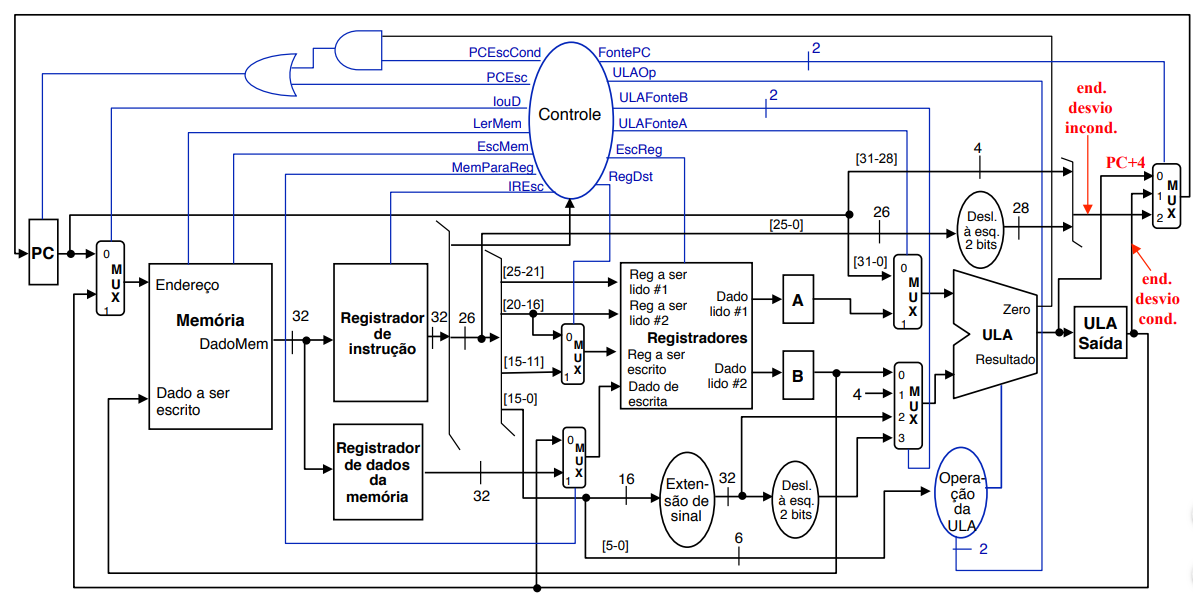
\includegraphics[scale=0.35]{circuito_mips.png} % leia abaixo
            \caption{Circuito do MIPS multiciclo.}
            \label{figura:mips}
        \end{figure}

        \subsection{Diagramas}

        \subsubsection{Transição de Estados}

        \begin{figure}[H]
            \centering % para centralizarmos a figura
            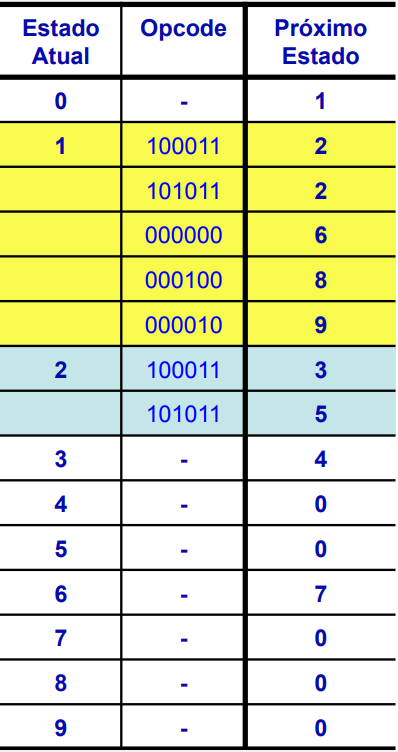
\includegraphics[scale=0.31]{transicao_estados.png} % leia abaixo
            \caption{Tabela de transição de estados.}
            \label{figura:mips}
        \end{figure}

        \subsubsection{Maquinas de Estado}

        \begin{figure}[H]
            \centering
            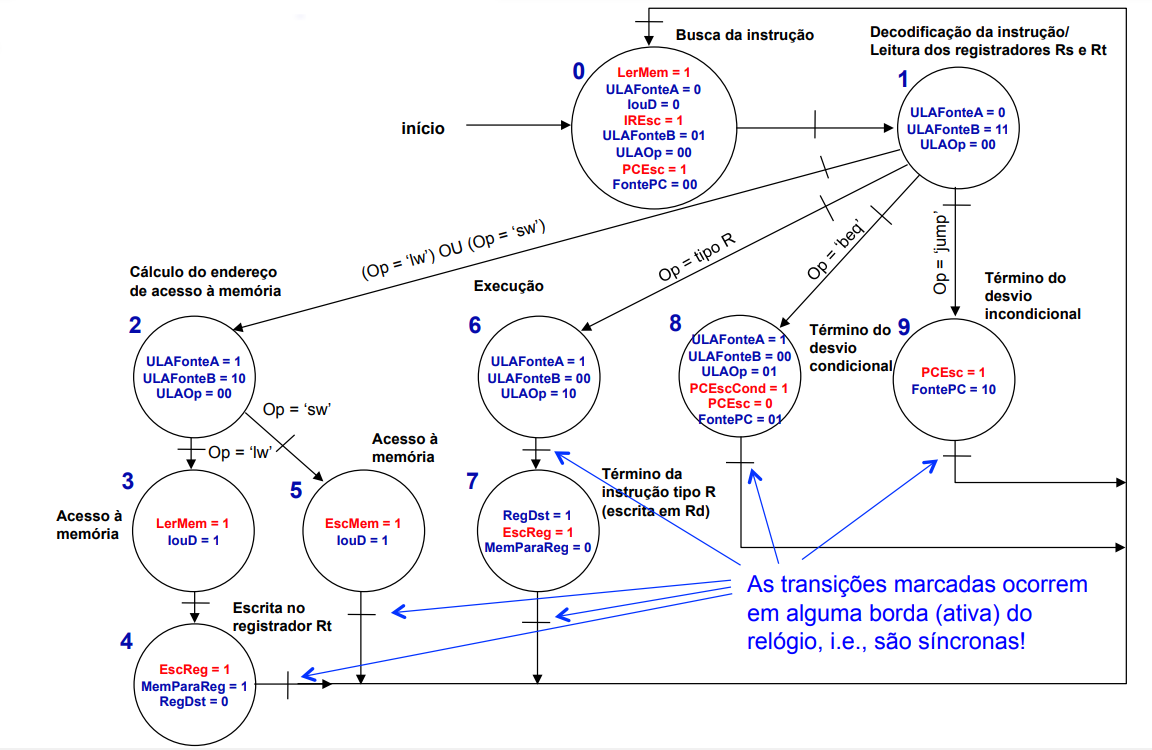
\includegraphics[scale=1.5]{maquina_estados.png}
            \caption{Maquina de estados do MIPS multiciclo.}
            \label{figura:maquina}
        \end{figure}

        \section{Resultados de atrasos}

        A seguir é apresentado os dados adquiridos após a compilação do MIPS
        multiciclo.

        \begin{figure}[H]
            \centering
            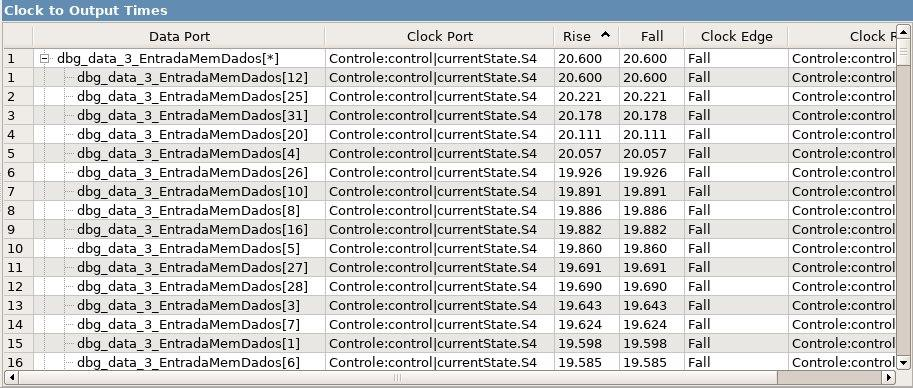
\includegraphics[width=\textwidth]{clock_to_output_times.jpg}
            \caption{Clock to Output Times.}
            \label{figura:mips}
        \end{figure}

        \begin{figure}[H]
            \centering
            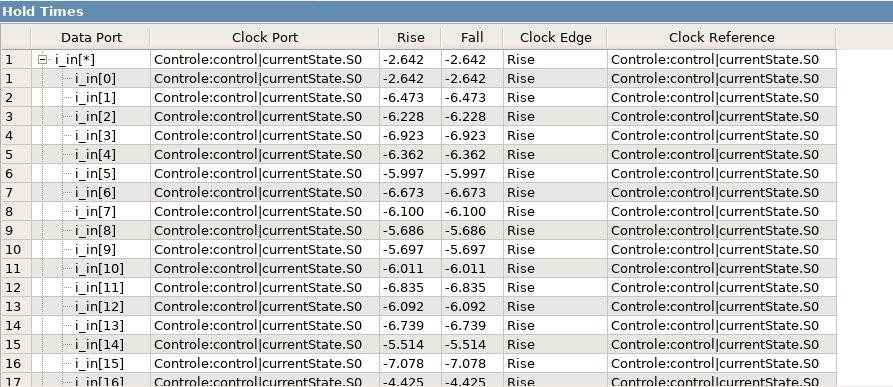
\includegraphics[width=\textwidth]{hold_times.jpg}
            \caption{Hold Times.}
            \label{figura:mips}
        \end{figure}

        \begin{figure}[H]
            \centering
            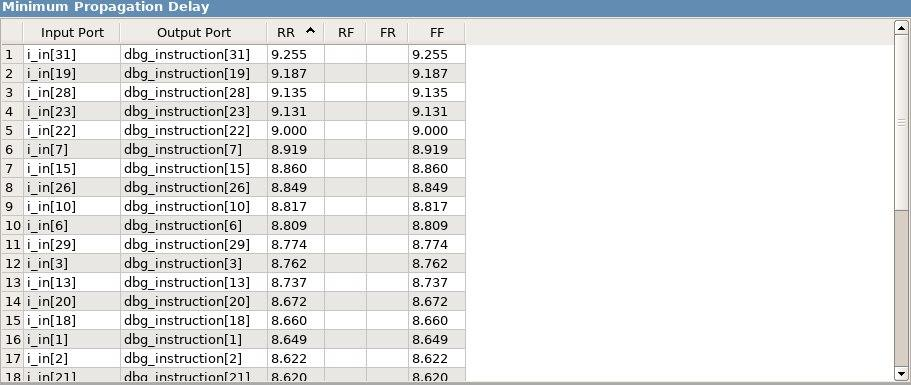
\includegraphics[width=\textwidth]{minimum_propagation_delay.jpg}
            \caption{Minimum Propagation Delay.}
            \label{figura:mips}
        \end{figure}

        \begin{figure}[H]
            \centering
            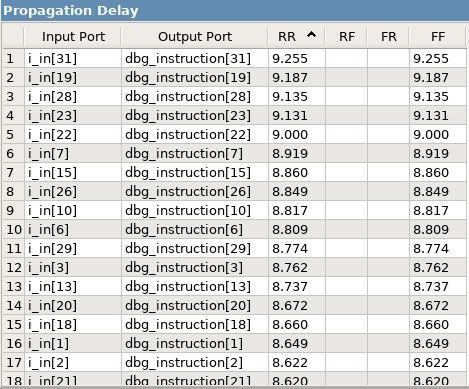
\includegraphics[width=\textwidth]{propagation_delay.jpg}
            \caption{Propagation Delay.}
            \label{figura:mips}
        \end{figure}

        \begin{figure}[H]
            \centering
            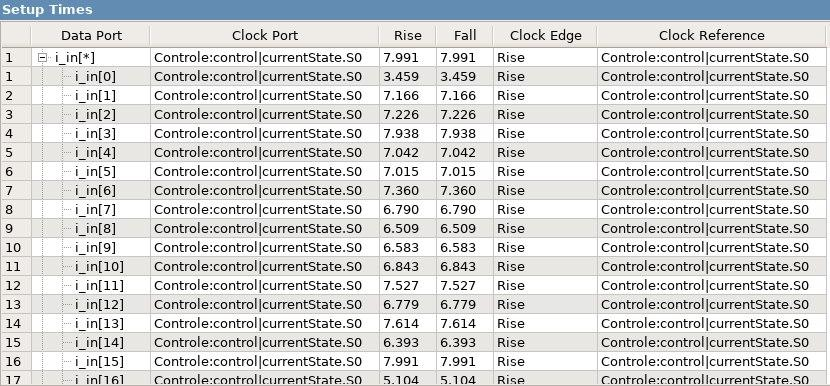
\includegraphics[width=\textwidth]{setup_times.jpg}
            \caption{Setup Times.}
            \label{figura:mips}
        \end{figure}


    \section{Utilização da placa}

    Utilizando os dados de compilação do Quartus, podemos ver que quanto ao uso
    de placa, o MIPS faz uso de uma quantidade muito pequena de registradores e
    funções combinacionais se comparado com o máximo suportado pela placa.
    Entretanto, o uso de pinos por parte dessa implementação é elevado,
    chegando a ultrapassar 50\% da capacidade total da placa.

    \begin{figure}[H]
        \centering
        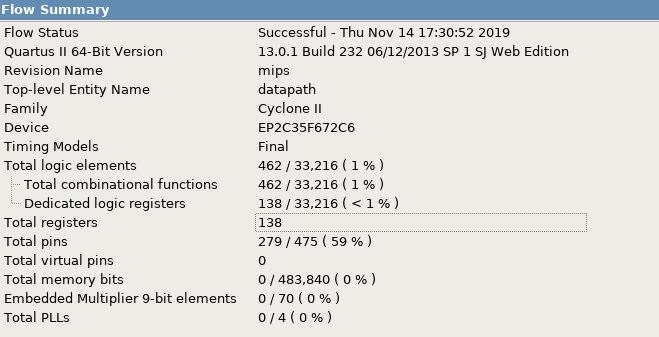
\includegraphics[width=\textwidth]{flow_summary.jpg}
        \caption{Flow Summary.}
        \label{figura:mips}
    \end{figure}

    \section{Discussão dos resultados}

    Durante os testes realizados com essa implementação do MIPS, a percepção
    geral do grupo é que uma implementação de um sistema digital complexo como
    um processador exige muito mais do que apenas a descrição do sistema em
    VHDL (ou outra linguagem de descrição de hardware). É necessário a
    aplicação de padrões de projeto e metodologias de teste mais ágeis do que o
    uso de arquivos .do com ModelSim.

    A simulação das instruções implementadas foi a parte mais complicada em
    questão de complexidade, além de não ter ficado muito claro como é feito o
    uso do Testbench, o software padrão de simulação da disciplina (ModelSim
    Altera) tem pouca documentação online e consome quantidades elevadas de
    recursos de hardware. Quanto maior a simulação, mais hardware consumido,
    até o ponto onde a simulação não consegue continuar, isso limitou
    significativamente o teste de um bloco grande de instruções e nos levou a
    optar por executar isoladamente cada instrução implementada.

    A criação e validação de uma memória de instruções também foi um problema,
    já que para forçar os sinais necessários para testes das instruções, esses
    testes deveriam ser inseridos diretamente na memória de instruções, porém a
    inserção de dados na memória de instruções da maneira atual só pode ser
    feita a partir de uma instrução (store word). Assim, foi decisão do grupo
    criar sinais "mímicos" para realizar os testes, estes sinais irão
    substituir a saída da memória de instruções e irão copiar a saída dos
    registradores mais importantes da implementação. Apesar de funcionar como
    uma metodologia de teste, para a implementação completa do MIPS, outra
    solução deve ser escolhida.

    As instruções que foram implementadas: Tipo R, Jump, Beq, Load Word, Store
    Word.  As instruções que foram validadas: Tipo R, Jump, Beq, Store Word

    A instrução Load Word não pode ser validada (apesar de ter sido
    implementada) justamente pela limitação de testes usando um sinal que imita
    a saída da memória de dados.

    \break{}

    \section{Testes}

    Instrução tipo R\: esse teste em específico realizou a instrução add a
    seguir, com os valores dos registradores base setados para 8 e 4,
    resultando em uma saída 12.

    \begin{figure}[H]
        \centering
        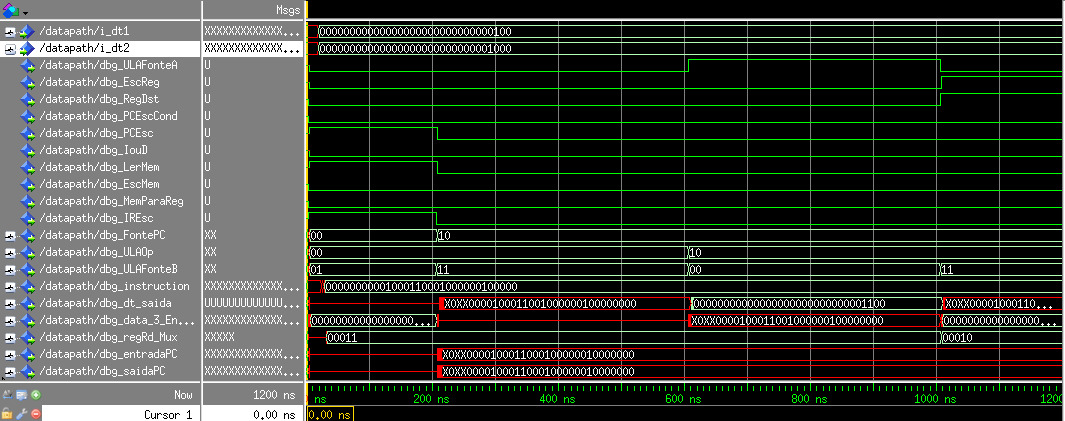
\includegraphics[width=\textwidth]{add_wave.jpg}
        \caption{Onda da simulação de uma instrução R}
        \label{figura:mips}
    \end{figure}

    Instrução tipo J\: esse teste em específico realizou a instrução jump a
    seguir, com um deslocamento do PC no valor de 24 unidades

    \begin{figure}[H]
        \centering
        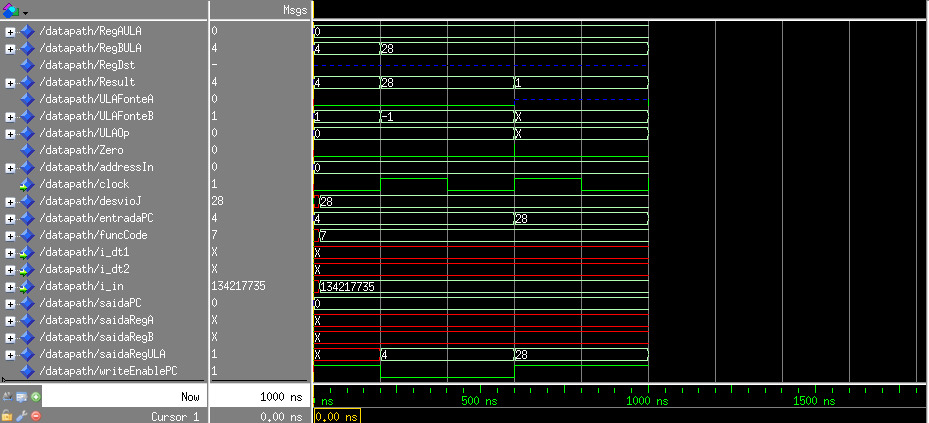
\includegraphics[width=\textwidth]{jump_wave.jpg}
        \caption{Onda da simulação de uma instrução J}
        \label{figura:mips}
    \end{figure}

    \section{Conclusões}

    \par Apesar de ser apenas uma versão resumida do MIPS, a implementação
    realizada contribui com a fixação de conhecimentos adquiridos tanto durante
    as aulas práticas quanto teóricas. Como processador com fins didáticos o
    MIPS cumpre um bom papel, sendo a compreensão do seu funcionamento
    intuitiva e simples.  Entretanto, o uso comercial do MIPS, que já foi
    explorado por algumas empresas, exige a implementação de todas as features
    do processador, incluindo também aumento nas memórias e quantidade de
    instruções.

    A gama limitada de instruções dessa versão do processador ainda consegue
    realizar blocos de instruções moderadamente complexos, mas pelo tamanho
    reduzido do banco de registradores e da memória RAM desse projeto, torna-se
    inviável escrever um programa completo para rodar nessa implementação
    reduzida.

\end{document}
